\documentclass{standalone}
\usepackage{tikz}
\usepackage{float}
\usepackage{amsmath}
\usepackage{lmodern}
\usepackage{amssymb}
\usetikzlibrary{calc}
\usetikzlibrary{hobby}
\usepackage{nicefrac}
\usetikzlibrary{decorations.markings, decorations.pathreplacing}
\usetikzlibrary{patterns, patterns.meta}
\usetikzlibrary{shapes,quotes, angles}
\usepackage{pgfplots}

\begin{document}
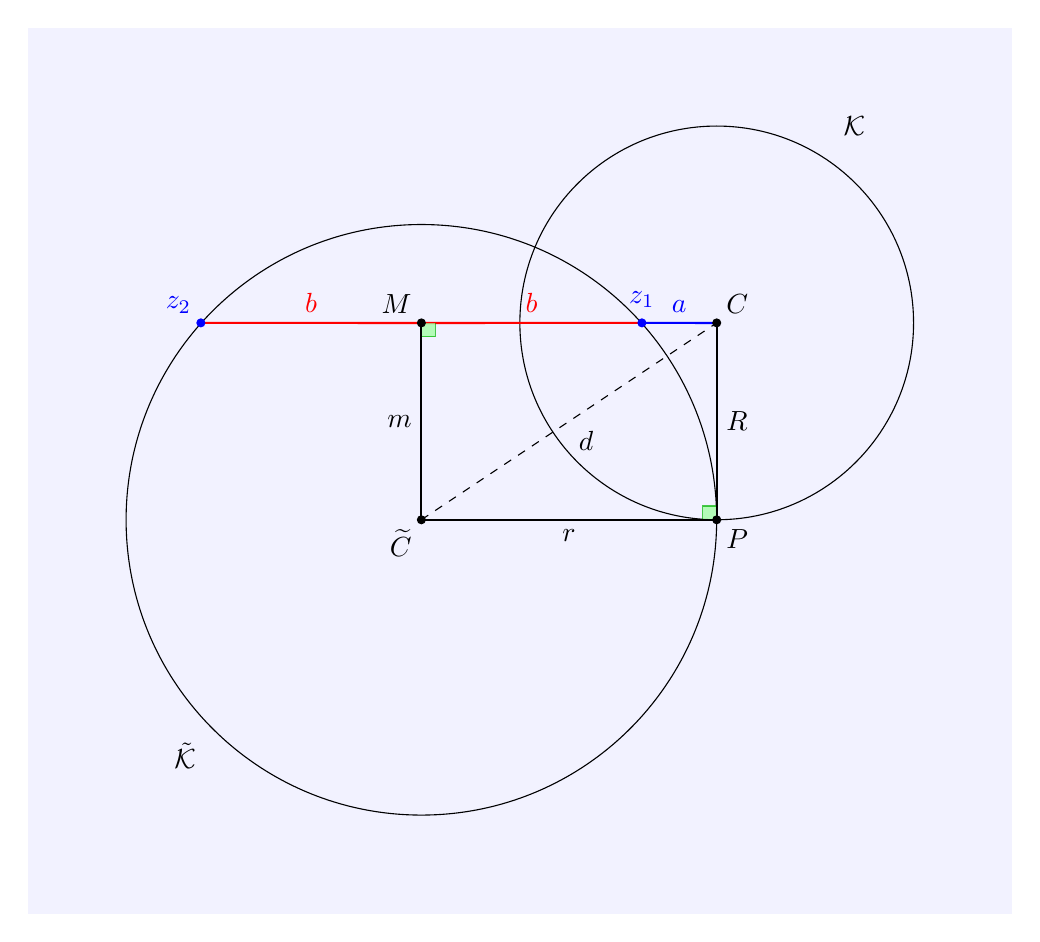
\begin{tikzpicture}[scale=2.5]

% Background for entire canvas
\fill[blue!5] (-2,-2) rectangle (3,2.5);

% Define rectangle corners
\coordinate (Ctilde) at (0,0);           % Bottom left
\coordinate (P) at (1.5,0);                % Bottom right
\coordinate (M) at (0,1);                % Top left
\coordinate (C) at (1.5,1);                % Top right

% Define radii based on geometry
\def\r{1.5}   % radius of left circle (from Ctilde to P)
\def\R{1}   % radius of right circle (from C to P)

% Draw rectangle
\draw[thick] (Ctilde) rectangle (C);

% Draw circles
\draw (Ctilde) circle[radius=\r];
\draw (C) circle[radius=\R];

% Diagonal
\draw[dashed] (Ctilde) -- (C) node[midway, below right] {$d$};

% Extend top edge to the left + coordinates
\coordinate (z2) at ($ (M) + (-1.12, 0) $); 
\draw[red, thick] (z2) -- (M) node[midway, above] {$b$};
\coordinate (z1) at ($ (M) + (+1.12, 0) $); 
\draw[red, thick] (M)--(z1) node[midway, above] {$b$};
\filldraw[blue] (z1) circle (0.02) node[above=2pt] {$z_1$};
\filldraw[blue] (z2) circle (0.02) node[above left] {$z_2$};

% z1 to C
\draw[blue, thick] (z1)--(C) node[midway, above] {$a$};



% Right angles
\draw pic["",draw=black, angle radius=5, angle eccentricity=1.2,color=green!70!black, fill=green!40, opacity=0.7] {right angle=C--M--Ctilde};
\draw pic["",draw=black, angle radius=5, angle eccentricity=1.2,color=green!70!black, fill=green!40, opacity=0.7] {right angle=C--P--Ctilde};

% Labels and points
\filldraw (Ctilde) circle (0.02) node[below left] {$\widetilde{C}$};
\filldraw (P) circle (0.02) node[below right] {$P$};
\filldraw (M) circle (0.02) node[above left] {$M$};
\filldraw (C) circle (0.02) node[above right] {$C$};

% Segment labels
\draw (Ctilde) -- (M) node[midway, left] {$m$};
\draw (C) -- (P) node[midway, right] {$R$};
\draw (Ctilde) -- (P) node[midway, below] {$r$};

\node at (-1.2, -1.2) {$\tilde{\mathcal{K}}$};
\node at (2.2, 2) {$\mathcal{K}$};

\end{tikzpicture}

\end{document}